\documentclass[11pt,english]{article}

%%%%%%%%%%%%%%%%%%%%%%%%%%%%%%%%%%%%%%%%%%%%%%%%%%%%%%%%%%%
% Packages
%%%%%%%%%%%%%%%%%%%%%%%%%%%%%%%%%%%%%%%%%%%%%%%%%%%%%%%%%%%

% paper size & margins
\usepackage{fullpage}
\usepackage[showframe=false,margin=1in]{geometry}
\parindent=0pt

% font management
\usepackage{relsize}
\usepackage[T1]{fontenc} % for properly hyphenating words with accented chars
\usepackage[latin1]{inputenc}
\usepackage{babel}

% math
\usepackage{amsmath, amsthm, amssymb}
\usepackage{textcomp}
\usepackage{stmaryrd}
\usepackage{upgreek}
\usepackage{bm}
\usepackage[linesnumbered,ruled,vlined]{algorithm2e}


% assorted
\usepackage{url}
\usepackage{breakurl}
\usepackage{xspace}
\usepackage{comment}
\usepackage{color}
\usepackage{afterpage}
\usepackage{tikz}

%%%%%%%%%%%%%%%%%%%%%%%%%%%%%%%%%%%%%%%%%%%%%%%%%%%%%%%%%%%
% Shortcuts
%%%%%%%%%%%%%%%%%%%%%%%%%%%%%%%%%%%%%%%%%%%%%%%%%%%%%%%%%%%
\newcommand{\hide}[1]{}
\DeclareMathOperator*{\argmin}{arg\,min}
\newtheorem{theorem}{Theorem}[section]
\newtheorem{corollary}{Corollary}[theorem]
\newtheorem{lemma}[theorem]{Lemma}

%%%%%%%%%%%%%%%%%%%%%%%%%%%%%%%%%%%%%%%%%%%%%%%%%%%%%%%%%%%
% Title / Author
%%%%%%%%%%%%%%%%%%%%%%%%%%%%%%%%%%%%%%%%%%%%%%%%%%%%%%%%%%%
\begin{document}

\title{CS7643: Deep Learning \\
Fall 2019\\ HW2 Solutions}
\author{James Hahn}
\maketitle

\setcounter{MaxMatrixCols}{25}
\setlength\arraycolsep{1pt}

%%%%%%%%%%%%%%%%%%%%%%%%%%%%%%%%%%%%%%%%%%%%%%%%%%%%%%%%%%%
% Body
%%%%%%%%%%%%%%%%%%%%%%%%%%%%%%%%%%%%%%%%%%%%%%%%%%%%%%%%%%%

\section{Convolution Basics}

\begin{enumerate}
	\item $A_1 = \tiny\begin{bmatrix}
	w_{(0, 0)} & w_{(0, 1)} & 0 & 0 & 0 & w_{(1, 0)} & w_{(1, 1)} & 0 & 0 & 0 & 0 & 0 & 0 & 0 & 0 & 0 & 0 & 0 & 0 & 0 & 0 & 0 & 0 & 0 & 0 \\
	0 & 0 & 0 & w_{(0, 0)} & w_{(0, 1)} & 0 & 0 & 0 & w_{(1, 0)} & w_{(1, 1)} & 0 & 0 & 0 & 0 & 0 & 0 & 0 & 0 & 0 & 0 & 0 & 0 & 0 & 0 & 0 \\
	0 & 0 & 0 & 0 & 0 & 0 & 0 & 0 & 0 & 0 & 0 & 0 & 0 & 0 & 0 & w_{(0, 0)} & w_{(0, 1)} & 0 & 0 & 0 & w_{(1, 0)} & w_{(1, 1)} & 0 & 0 & 0 \\
	0 & 0 & 0 & 0 & 0 & 0 & 0 & 0 & 0 & 0 & 0 & 0 & 0 & 0 & 0 & 0 & 0 & 0 & w_{(0, 0)} & w_{(0, 1)} & 0 & 0 & 0 & w_{(1, 0)} & w_{(1, 1)} \\
	\end{bmatrix}_{4x25}$ 
	
	This above matrix $A_1$ assumes input $X$ has the zero-padding elements placed in it.
	
	$A_2 = \tiny\begin{bmatrix}
	w_{(1, 1)} & 0 & 0 & 0 & 0 & 0 & 0 & 0 & 0 \\
	0 & 0 & w_{(1, 0)} & 0 & 0 & 0 & 0 & 0 & 0 \\
	0 & 0 & 0 & 0 & 0 & 0 & w_{(0, 1)} & 0 & 0 \\
	0 & 0 & 0 & 0 & 0 & 0 & 0 & 0 & w_{(0, 0)} \\
	\end{bmatrix}_{4x9}$ 
	
	Meanwhile, matrix $A_2$ assumes input $X$ doesn't have the zero-padding elements placed in the vector.
	
	Both matrices achieve the desired goal in this question, it just depends on how $X$ is implemented, which is not specified by the question itself.
	\pagebreak
	\item $A = \begin{bmatrix}
	w_{(0, 0)} & 0 & 0 & 0 \\
	w_{(0, 1)} & 0 & 0 & 0 \\
	0 & w_{(0, 0)} & 0 & 0 \\
	0 & w_{(0, 1)} & 0 & 0 \\
	w_{(1, 0)} & 0 & 0 & 0 \\
	w_{(1, 1)} & 0 & 0 & 0 \\
	0 & w_{(1, 0)} & 0 & 0 \\
	0 & w_{(1, 1)} & 0 & 0 \\
	0 & 0 & w_{(0, 0)} & 0 \\
	0 & 0 & w_{(0, 1)} & 0 \\
	0 & 0 & 0 & w_{(0, 0)} \\
	0 & 0 & 0 & w_{(0, 1)} \\
	0 & 0 & w_{(1, 0)} & 0 \\
	0 & 0 & w_{(1, 1)} & 0 \\
	0 & 0 & 0 & w_{(1, 0)} \\
	0 & 0 & 0 & w_{(1, 1)}
	\end{bmatrix}_{16x4}$\\
	
	One of the TA's on Piazza stated $X$ should be transposed in this question, meaning $X$ would be 4x1. So, $Y = AX$ results in a 16x1 output matrix, indicating the matrix is upsampled from a 2x2 matrix to a 4x4 matrix.
	
	\pagebreak
	\item $A = \begin{bmatrix}
	w_{(0, 0)} & 0 & 0 & 0 \\
	0 & w_{(0, 0)} & 0 & 0 \\
	0 & 0 & w_{(0, 0)} & 0 \\
	0 & 0 & 0 & w_{(0, 0)} \\
	w_{(0, 1)} & 0 & 0 & 0 \\
	0 & w_{(0, 1)} & 0 & 0 \\
	0 & 0 & w_{(0, 1)} & 0 \\
	0 & 0 & 0 & w_{(0, 1)} \\
	w_{(1, 0)} & 0 & 0 & 0 \\
	0 & w_{(1, 0)} & 0 & 0 \\
	0 & 0 & w_{(1, 0)} & 0 \\
	0 & 0 & 0 & w_{(1, 0)} \\
	w_{(1, 1)} & 0 & 0 & 0 \\
	0 & w_{(1, 1)} & 0 & 0 \\
	0 & 0 & w_{(1, 1)} & 0 \\
	0 & 0 & 0 & w_{(1, 1)}
	\end{bmatrix}_{16x4}$ \\
	$Y = AX^T = \begin{bmatrix}
	w_{(0, 0)}x_{(0, 0)} \\
	w_{(0, 0)}x_{(0, 1)} \\
	w_{(0, 0)}x_{(1, 0)} \\
	w_{(0, 0)}x_{(1, 1)} \\
	w_{(0, 1)}x_{(0, 0)} \\
	w_{(0, 1)}x_{(0, 1)} \\
	w_{(0, 1)}x_{(1, 0)} \\
	w_{(0, 1)}x_{(1, 1)} \\
	w_{(1, 0)}x_{(0, 0)} \\
	w_{(1, 0)}x_{(0, 1)} \\
	w_{(1, 0)}x_{(1, 0)} \\
	w_{(1, 0)}x_{(1, 1)} \\
	w_{(1, 1)}x_{(0, 0)} \\
	w_{(1, 1)}x_{(0, 1)} \\
	w_{(1, 1)}x_{(1, 0)} \\
	w_{(1, 1)}x_{(1, 1)}
	\end{bmatrix}_{16x1}$\\\\
	Y is the result of the convolutional layer with kernel size (4, 1, 1, 1)\\
	If we use the transposed convolutional layer of size (1, 1, 2, 2) and weights $W = \begin{bmatrix}
	w_{(0, 0)} & w_{(0, 1)} & w_{(1, 0)} & w_{(1, 1)}
	\end{bmatrix}^T$, we can create convolutional matrix $W'$ as follows: \\
	$W' = \begin{bmatrix}
	w_{(0, 0)} & 0 & 0 & 0 \\
	0 & w_{(0, 1)} & 0 & 0 \\
	0 & 0 & w_{(1, 0)} & 0 \\
	0 & 0 & 0 & w_{(1, 1)} \\
	w_{(0, 0)} & 0 & 0 & 0 \\
	0 & w_{(0, 1)} & 0 & 0 \\
	0 & 0 & w_{(1, 0)} & 0 \\
	0 & 0 & 0 & w_{(1, 1)} \\
	w_{(0, 0)} & 0 & 0 & 0 \\
	0 & w_{(0, 1)} & 0 & 0 \\
	0 & 0 & w_{(1, 0)} & 0 \\
	0 & 0 & 0 & w_{(1, 1)} \\
	w_{(0, 0)} & 0 & 0 & 0 \\
	0 & w_{(0, 1)} & 0 & 0 \\
	0 & 0 & w_{(1, 0)} & 0 \\
	0 & 0 & 0 & w_{(1, 1)}
	\end{bmatrix}_{16x4}$\\\\
	Then we get the following:\\\\
	$Y' = W'X = \begin{bmatrix}
	w_{(0, 0)}x_{(0, 0)} \\
	w_{(0, 1)}x_{(0, 0)} \\
	w_{(1, 0)}x_{(0, 0)} \\
	w_{(1, 1)}x_{(0, 0)} \\
	w_{(0, 0)}x_{(0, 1)} \\
	w_{(0, 1)}x_{(0, 1)} \\
	w_{(1, 0)}x_{(0, 1)} \\
	w_{(1, 1)}x_{(0, 1)} \\
	w_{(0, 0)}x_{(1, 0)} \\
	w_{(0, 1)}x_{(1, 0)} \\
	w_{(1, 0)}x_{(1, 0)} \\
	w_{(1, 1)}x_{(1, 0)} \\
	w_{(0, 0)}x_{(1, 1)} \\
	w_{(0, 1)}x_{(1, 1)} \\
	w_{(1, 0)}x_{(1, 1)} \\
	w_{(1, 1)}x_{(1, 1)}
	\end{bmatrix}_{16x1}$\\\\
	
	%\begin{bmatrix}
	%w_{(0, 0)}x_{(0, 0)} & w_{(0, 0)}x_{(0, 1)} & w_{(0, 0)}x_{(1, 0)} & w_{(0, %0)}x_{(1, 1)} \\
	%w_{(0, 1)}x_{(0, 0)} & w_{(0, 1)}x_{(0, 1)} & w_{(0, 1)}x_{(1, 0)} & w_{(0, %1)}x_{(1, 1)} \\
	%w_{(1, 0)}x_{(0, 0)} & w_{(1, 0)}x_{(0, 1)} & w_{(1, 0)}x_{(1, 0)} & w_{(1, %0)}x_{(1, 1)} \\
	%w_{(1, 1)}x_{(0, 0)} & w_{(1, 1)}x_{(0, 1)} & w_{(1, 1)}x_{(1, 0)} & w_{(1, %1)}x_{(1, 1)} \\
	%\end{bmatrix}_{4x4}$
	
	As such, if we compare $Y$ with $Y'$, we see they are identical. On a side note, please ignore the spacing between the columns of the matrices. There are indeed 16 elements in that matrix, but I had to make the column margins small to fit the $4x25$ matrix in question 1.
\end{enumerate}
\pagebreak

\section{Logic and XOR}

\begin{enumerate}
	\item $w_{AND} = [0.5, 0.5]$ and $b_{AND} = -1$ \\\\
	To show these weights and bias are valid, we see the following: \\\\
	$x_1 = 0, x_2 = 0: [0.5, 0.5][0, 0]^T - 1 = 0 - 1 = -1 < 0 \implies f_{AND}(x) = 0 \\
	x_1 = 0, x_2 = 1: [0.5, 0.5][0, 1]^T - 1 = 0.5 - 1 = -0.5 < 0 \implies f_{AND}(x) = 0 \\
	x_1 = 1, x_2 = 0: [0.5, 0.5][1, 0]^T - 1 = 0.5 - 1 = -0.5 < 0 \implies f_{AND}(x) = 0 \\
	x_1 = 1, x_2 = 1: [0.5, 0.5][1, 1]^T - 1 = 1.0 - 1 = 0 \geq 0 \implies f_{AND}(x) = 1$ \pagebreak	
	\item $w_{OR} = [0.5, 0.5]$ and $b_{OR} = -0.5$ \\\\
	To show these weights and bias are valid, we see the following: \\\\
	$x_1 = 0, x_2 = 0: [0.5, 0.5][0, 0]^T - 0.5 = 0 - 0.5 = -0.5 < 0 \implies f_{OR}(x) = 0 \\
	x_1 = 0, x_2 = 1: [0.5, 0.5][0, 1]^T - 0.5 = 0.5 - 0.5 = 0 \geq 0 \implies f_{OR}(x) = 1 \\
	x_1 = 1, x_2 = 0: [0.5, 0.5][1, 0]^T - 0.5 = 0.5 - 0.5 = 0 \geq 0 \implies f_{OR}(x) = 1 \\
	x_1 = 1, x_2 = 1: [0.5, 0.5][1, 1]^T - 0.5 = 1.0 - 0.5 = 0.5 \geq 0 \implies f_{OR}(x) = 1$
	\pagebreak
	\item Refer to the below graphic.\\\\
	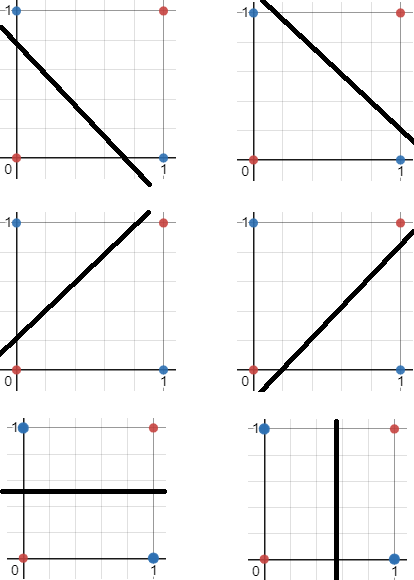
\includegraphics[scale=0.5]{2-2.png} \\
	We observe, when plotting the four data points (class-colored by red and blue), there are six general combinations of linear functions that can be used to separate these samples. However, all six functions fail to perfectly separate the two classes. There is always at least one data point that is left over from another class. It is quite obvious to see XOR is not a linearly separable function.
\end{enumerate}
\pagebreak

\section{Piecewise Linearity}

\begin{enumerate}
	\item $h(x) = h(1) \\
	= W^{(3)}max\{0, W^{(2)}max\{0, W^{(1)}x + b^{(1)}\} + b^{(2)}\} + b^{(3)} \\
	=  \begin{bmatrix} 1 & 1 \end{bmatrix}max\{0,  \begin{bmatrix} 1 & 1 \\ 1 & 1 \end{bmatrix}max\{0, \begin{bmatrix} 0.5 \\ 0.5 \end{bmatrix}(1) +  \begin{bmatrix} 0 \\ 1 \end{bmatrix}\} +  \begin{bmatrix} 0 \\ 0 \end{bmatrix}\} + 1 \\
	= \begin{bmatrix} 1 & 1 \end{bmatrix}max\{0,  \begin{bmatrix} 1 & 1 \\ 1 & 1 \end{bmatrix}\begin{bmatrix} 0.5 \\ 1.5 \end{bmatrix} +  \begin{bmatrix} 0 \\ 0 \end{bmatrix}\} + 1 \\
	= \begin{bmatrix} 1 & 1 \end{bmatrix}\begin{bmatrix} 2 \\ 2 \end{bmatrix} + 1 \\
	= 4 + 1 \\
	= 5$ \\
	In order for $Wx + b = h(x)$ to hold, you can set $W = 3$ and $b = 2$. In this case, $\frac{dh}{dx} = \frac{d}{dx} (Wx + b) = W = 3$. \pagebreak
	\item  $h(x) = h(1) \\
	= W^{(3)}max\{0, W^{(2)}max\{0, W^{(1)}x + b^{(1)}\} + b^{(2)}\} + b^{(3)} \\
	=  \begin{bmatrix} 1 & 1 \end{bmatrix}max\{0,  \begin{bmatrix} 1 & 1 \\ 1 & 1 \end{bmatrix}max\{0, \begin{bmatrix} 0.5 \\ 0.5 \end{bmatrix}(-1) +  \begin{bmatrix} 0 \\ 1 \end{bmatrix}\} +  \begin{bmatrix} 0 \\ 0 \end{bmatrix}\} + 1 \\
	= \begin{bmatrix} 1 & 1 \end{bmatrix}max\{0,  \begin{bmatrix} 1 & 1 \\ 1 & 1 \end{bmatrix}\begin{bmatrix} 0 \\ 0.5 \end{bmatrix} +  \begin{bmatrix} 0 \\ 0 \end{bmatrix}\} + 1 \\
	= \begin{bmatrix} 1 & 1 \end{bmatrix}\begin{bmatrix} 0.5 \\ 0.5 \end{bmatrix} + 1 \\
	= 1 + 1 \\
	= 2$ \\
	In order for $Wx + b = h(x)$ to hold, you can set $W = -1$ and $b = 1$. In this case, $\frac{dh}{dx} = \frac{d}{dx} (Wx + b) = W = -1$. \pagebreak
	\item $h(x) = h(1) \\
	= W^{(3)}max\{0, W^{(2)}max\{0, W^{(1)}x + b^{(1)}\} + b^{(2)}\} + b^{(3)} \\
	=  \begin{bmatrix} 1 & 1 \end{bmatrix}max\{0,  \begin{bmatrix} 1 & 1 \\ 1 & 1 \end{bmatrix}max\{0, \begin{bmatrix} 0.5 \\ 0.5 \end{bmatrix}(-0.5) +  \begin{bmatrix} 0 \\ 1 \end{bmatrix}\} +  \begin{bmatrix} 0 \\ 0 \end{bmatrix}\} + 1 \\
	= \begin{bmatrix} 1 & 1 \end{bmatrix}max\{0,  \begin{bmatrix} 1 & 1 \\ 1 & 1 \end{bmatrix}\begin{bmatrix} 0 \\ 0.75 \end{bmatrix} +  \begin{bmatrix} 0 \\ 0 \end{bmatrix}\} + 1 \\
	= \begin{bmatrix} 1 & 1 \end{bmatrix}\begin{bmatrix} 0.75 \\ 0.75 \end{bmatrix} + 1 \\
	= 1.5 + 1 \\
	= 2.5$ \\
	In order for $Wx + b = h(x)$ to hold, you can set $W = -2$ and $b = 0.5$. In this case, $\frac{dh}{dx} = \frac{d}{dx} (Wx + b) = W = -2$.
\end{enumerate}
\pagebreak

\section{Depth - Composing Linear Pieces}

\begin{enumerate}
	\item First, let's simplify this problem and set $d = 1$. In this case, there is one input neuron $x$ and one output neuron $y$. The one weight connecting the two neurons has value 2 with bias -1. So, $y$ can be represented as $f_1(x) = y_1 = |2x_1 - 1|$. In this scenario, $x$ has two regions $R_i$ that map to $O = (0, 1)$ and they are $R = \{(0, \frac{1}{2}), (\frac{1}{2}, 1)\}$. Now, it is trivial to expand this scenario through induction. For a given $x \in \mathbb{R}^d$, $y_i = |2x_i - 1|$. Therefore, for all $d$ input neurons, there are 2 input regions that map to output region $O$ as defined above. In the case of 2 input neurons and 2 output neurons, $x_1$ can map to two regions and $x_2$ can map to two regions. It follows that there are $4 = 2^d$ input regions $R_i$ that map to output region $O$ since $x_1, x_2$ can each take one of the two input regions. When $d = 3$, each input neuron $x_1, x_2, x_3$ can choose one of two regions each, resulting in $2^d = 2^3 = 8$ input regions. If we assume $x \in \mathbb{R}^{d-1}$ identifies $2^{d-1}$ input regions, then $x \in \mathbb{R}^d$ will identify $2\cdot 2^{d-1} = 2^d$. The multiplicative factor of 2 comes from $x_d$ having 2 input regions to choose from. 
	
	As such, this pattern follows and we find given an input $x \in \mathbb{R}^d$ and output $y \in \mathbb{R}^d$, there are $2^d$ input regions that map to the hypercube $O = (0, 1)^d$.  \qed \pagebreak
	\item To simplify this problem, let $d = 1$. This means we have one input neuron $x_1$, one hidden neuron $z_1$, and one output neuron $y_1$. If $g(\cdot) = g(x)$ maps $n_g$ regions onto $(0, 1)$, then $x_1$ can pick any of those $n_g$ regions for its mapping. Now, when we choose $x_1$ in any one of these regions, $x_1 \in R_{n_{g_i}}$, it maps to $(0, 1)$, which is the input interval we need for $f$, which maps $(0, 1)$ to $(0, 1)$. If there are $n_f$ regions in $(0, 1)$ that map to $(0, 1)$ for $f$, that means for all $n_g$ regions that $x_1$ can choose from, once we compute $g(x_1)$, there are then $n_f$ regions that map $g(x_1)$ to $(0, 1)$. As such, in this $d = 1$ example, there are $n_gn_f$ possible regions that $f \circ g(x_1)$ identifies onto $(0, 1)$. 
	
	It is trivial to see this rule follows for higher values of $d$. This is because $g(x)$ is a bijection onto $f$ and $f(x)$ is a bijection onto $O$. As such, for all $n_g$ regions in $g(x)$ that map onto $f$, there are $n_f$ regions in $f(x)$ that map onto $O$. Therefore, the total number of input regions that $f \circ g(\cdot)$ identifies onto $(0, 1)^d$ is $n_gn_f$. \qed \pagebreak
	\item First, observe that\\\\
	 $h_1(x) = |W_1x + b_1| \\
	 h_2(h_1(x)) = |W_2h1(x) + b2| \\
	 \dots \\
	 h_L(h_{L-1}) = |W_Lh_{L-1} + b_L| = h_L \circ h_{L-1} \dots \circ h_2 \circ h_1(x)$ \\\\
	 We want to show $h_L$ identifies $2^{Ld}$ regions. First, from question 4.1, we proved the absolute value function identifies $2^d$ regions onto $(0, 1)$. Second, in question 4.2, we proved if $h_1$ maps $n_{h_1}$ regions onto $h_2$ and $h_2$ maps $n_{h_2}$ regions onto $h_3$, then $h_1$ maps $n_{h_1}n_{h_2}$ regions onto $h_3$. \\
	 To prove this by induction, assume we have $L$ layers of our network, represented by $f(x) = h_L \circ h_{L-1} \dots \circ h_2 \circ h_1(x)$. The result from question 4.1 is our base case. So, if we assume the $(L-1)^{th}$ layer, $h_{L-1}$, identifies $2^{(L-1)d}$ regions of our input (using result from 4.1), then $h_L(h_{L-1})$ maps $2^d 2^{(L-1)d} = 2^{Ld}$ regions of the input (using result from 4.2). As such, we have shown a series of $L$ layers identifies $2^{Ld}$ input regions. \qed
\end{enumerate}

\end{document}
